% %
% LAYOUT_E.TEX - Short description of REFMAN.CLS
%                                       99-03-20
%
%  Updated for REFMAN.CLS (LaTeX2e)
%
\documentclass[twoside,a4paper]{refart}
\usepackage{fancyvrb}
\usepackage{makeidx}
\usepackage{ifthen}
\usepackage{graphicx}
\usepackage{hyperref}
\hypersetup{
    colorlinks,
    citecolor=black,
    filecolor=black,
    linkcolor=blue,
    urlcolor=black
}
% ifthen wird vom Bild von N.Beebe gebraucht!

\def\bs{\char'134 } % backslash in \tt font.
\newcommand{\ie}{i.\,e.,}
\newcommand{\eg}{e.\,g..}
\DeclareRobustCommand\cs[1]{\texttt{\char`\\#1}}

\title{WARP User's Guide}
\author{Ryan M. Bergmann \thanks{ryanmbergmann@gmail.com} \\
Kelly L. Rowland \thanks{krowland@berkeley.edu}\\
v 1.0,  April 2016}

\date{}
\emergencystretch1em  %

\pagestyle{myfootings}
\markboth{WARP User's Guide}%
                {WARP User's Guide}

\makeindex 

\setcounter{tocdepth}{2}

\begin{document}

\maketitle

%\begin{abstract}
%
%This is the user guide for WARP.
%
%\end{abstract}

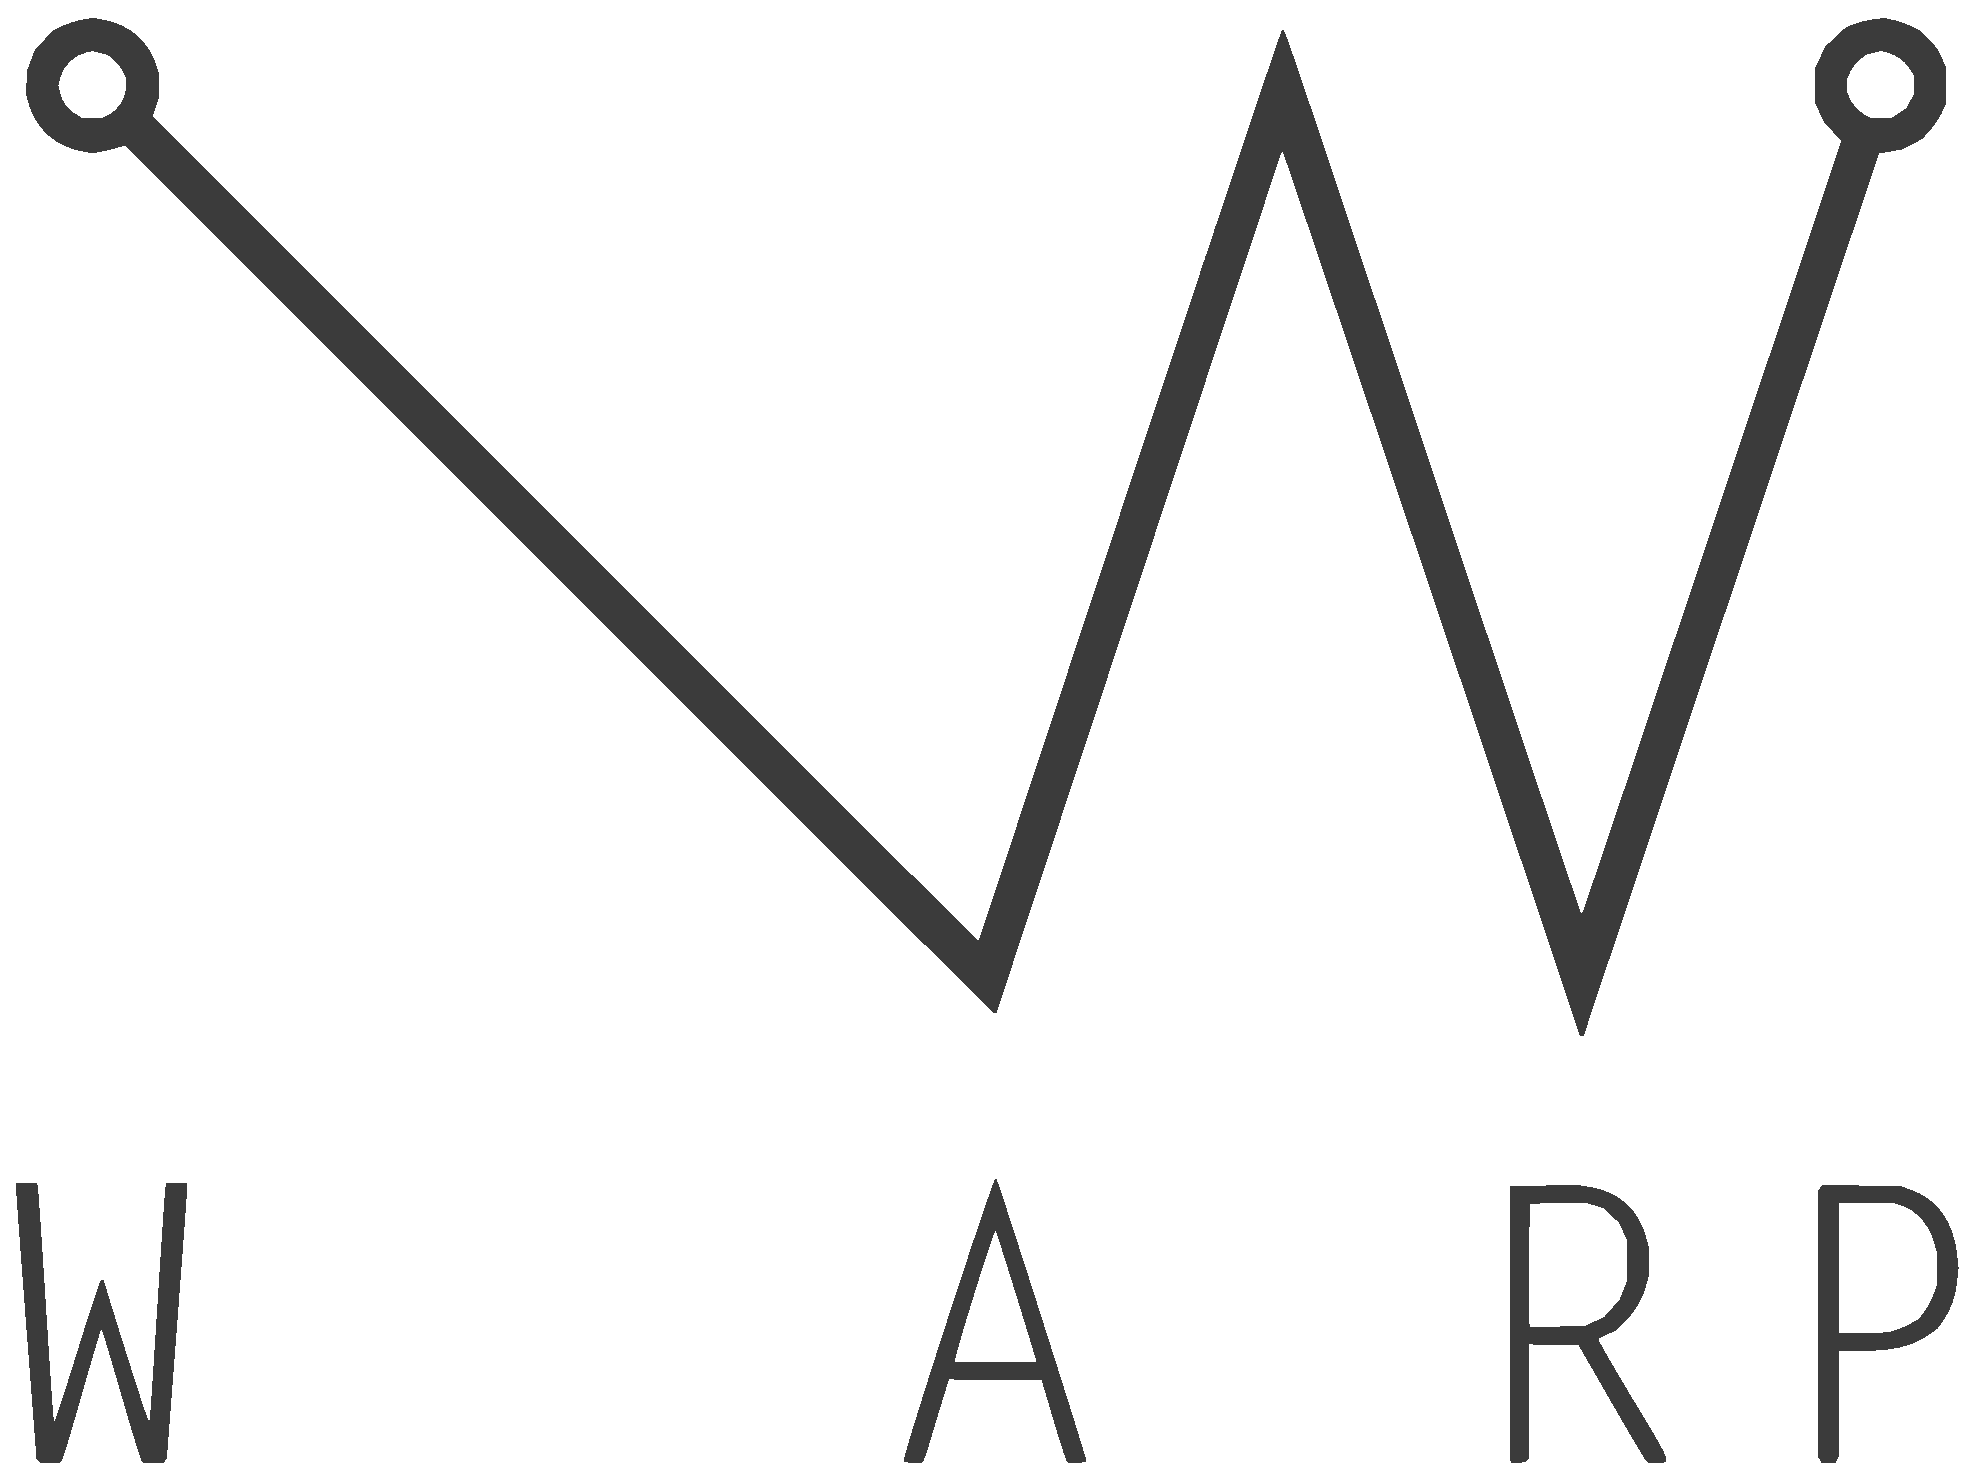
\includegraphics[width=\linewidth]{graphics/warp-vec.eps}

\vspace*{\fill} % this vertically centers the next paragraph

This user's guide is meant to introduce a user to the way in which WARP executes and how its top-level 
functionality can be used to solve neutron transport problems.  For more detailed information about the 
algorithms WARP uses, please refer to article ``Algorithmic choices in WARP - A framework for continuous 
energy Monte Carlo neutron transport in general 3D geometries on GPUs'' in Annals of Nuclear Engineering 
(doi:10.1016/j.anucene.2014.10.039) and ``Relative Performance and Accuracy of Neutron Criticality Calculations Performed by WARP- A Framework for Continuous Energy Monte Carlo Neutron Transport in General 3D Geometries on GPUs'' in Annals of Nuclear Engineering (doi: XXX).

\vfill


\newpage
\tableofcontents
\newpage


%%%%%%%%%%%%%%%%%%%%%%%%%%%%%%%%%%%%%%%%%%%%%%%%%%%%%%%%%%%%%%%%%%%%

\section{An Introduction to WARP}

WARP is a C\texttt{++} library that contains a set of classes and data structures that allow Monte Carlo 
neutron transport to be performed using graphics processing units (GPUs).  It is written to scale well and
execute efficiently on a single GPU.

Typical CPU codes track a single neutron life, from cradle to grave, marking its interactions along the 
way. WARP does things a little differently.  WARP applies the main transport loop to an entire (preferably
large) set of neutrons instead of a single neutron.  The parallelism in WARP comes from acting on many 
similar pieces of data concurrently instead of executing many, possibly dissimilar tasks concurrently.

\begin{figure}[h!] 
  \centering
    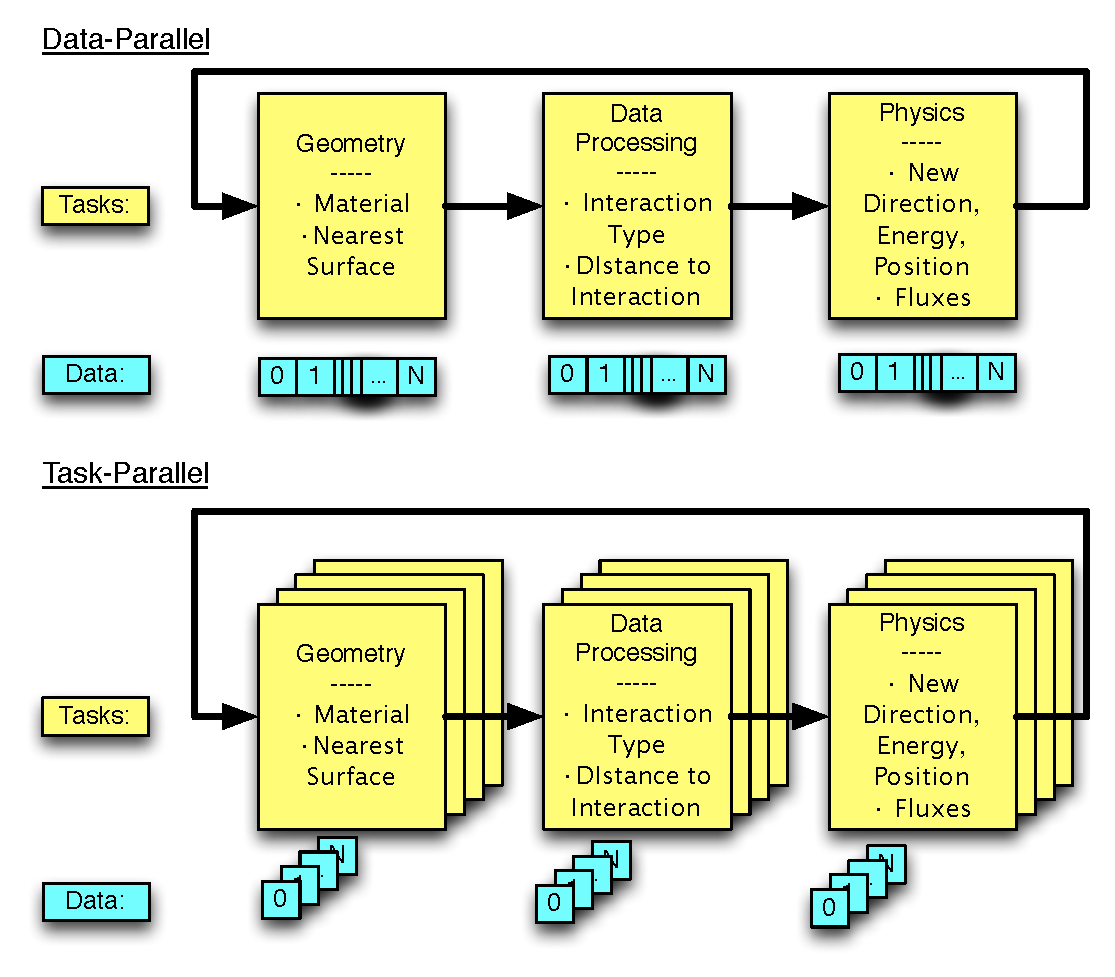
\includegraphics[width=\textwidth]{graphics/datavtask.pdf}
     \caption{Data-parallel neutron trasport loop vs. a task-parallel transport loop for transporting N neutrons in parallel.  \label{datavtask} }
\end{figure}

\section{Dependencies of WARP}

WARP has the following dependencies:

\begin{description}

\item[C\texttt{++} compiler]\index{C\texttt{++} compiler}
Compilers are programs that convert source code written in a given programming language (C\texttt{++}, in 
this case) into machine language that is used by a computer's processor.

One commonly used C\texttt{++} compiler is \texttt{gcc}, which can be downloaded at 
\url{https://gcc.gnu.org/releases.html}. Installation instructions can be found at 
\url{https://gcc.gnu.org/install/}.

\item[CMake]\index{CMake}$\ge$ 2.8.10 \\
CMake is ``an extensible, open-source system that manages the build process in an operating system and in
a compiler-independent manner."

CMake is free and can be downloaded here: \url{https://cmake.org/download/}.

Instructions for installing CMake on various operating systems can be found at 
\url{https://cmake.org/install/}.
  
\item[NVIDIA CUDA]\index{NVIDIA CUDA}$\ge$ 5.0 \\
CUDA (``Compute Unified Device Architecture") is a parallel computing platform and programming model 
invented by NVIDIA to utilize the power of the GPU. \textbf{Your computer must include a CUDA-enabled 
GPU in order to install and use CUDA.}

The latest version of CUDA can be downloaded here: \url{https://developer.nvidia.com/cuda-downloads}.

Documentation for the CUDA Toolkit can be found at \url{http://docs.nvidia.com/cuda/index.html}.

\item[NVIDIA OptiX]\index{NVIDIA OptiX}$\ge$ 3.0.1 \\
OptiX is a software development kit developed by NVIDIA for ray tracing performance on GPUs; it provides a
framework for accessing the GPU's ray tracing capabilities.

Instructions for and information about downloading OptiX are here: \url{https://developer.nvidia.com/download}.

\item[CUDPP]\index{CUDPP}$\ge$ 2.1 \\
CUDPP (``CUDA Data Parallel Primitives") is a library of data-parallel algorithm primitives such as 
parallel sort, can, and reduction.

CUDPP can be downloaded at \url{http://cudpp.github.io/} with documentation available at 
\url{http://cudpp.github.io/cudpp/2.2/}.

\item[SWIG]\index{SWIG}$\ge$ 1.3.40 \\
SWIG is an interface compiler that connects programs written in C/C\texttt{++} with scripting languages
like Python; it is used for the WARP Python interface.

SWIG can be downloaded at \url{http://www.swig.org/download.html}.

\item[Google Test]\index{GoogleTest}$\ge$ 1.7.0 \\
Google Test is a framework for writing C\texttt{++} tests on a variety of platforms. The WARP test suite
is built on Google Test.

Google Test can be downloaded here: \url{https://code.google.com/p/googletest/downloads/list}.

Documentation can be found at \url{https://code.google.com/p/googletest/wiki/Documentation}.

\item[ACE formatted nuclear cross section data]\index{ACE formatted nuclear cross section data}
$\ge$ ENDF/B-VII.1 \\
ACE (``a compact ENDF") formatted data is nuclear cross section data is tabulated such that it is read in 
by many Monte Carlo codes; the data includes cross sections as well as angular and energy distributions 
used in neutron scattering and fission.

ACE formatted files can be downloaded at \url{http://www.nndc.bnl.gov/endf/b7.1/acefiles.html} and are 
also included with releases of the MCNP and Serpent from RSICC (rsicc url).

\end{description}

!!!! standalone now, so this section needs ot be modified!

PyNE (``Python for Nuclear Engineering", \url{http://pyne.io/}) is an open-source toolkit for calculations related to nuclear
engineering.  WARP has taken the ``ace'' module of PyNE and modified it to be a stand-alone Python module independent of of PyNE.  Legally, this is acceptable since WARP is released as open-source software under the same BSD license under which PyNE is released.

\section{Building WARP}

WARP can be compiled with CMake. To build WARP, follow these steps:

\begin{enumerate}
\item{Install git if it isn't already installed on your system (currently only *nix distributions and OSX are supported)}
\item{Download WARP from GitHub.  On the command line: \texttt{git clone blah} }
\item{Create an empty directory outside of the WARP source code folder and navigate into that directory.}
\item{In the terminal, enter \texttt{ccmake /path/to/warp}, where the path is the absolute or relative 
path to the WARP source code directory.}
\item{Configure the code and set \texttt{OptiX\_ROOT\_DIR} and \texttt{CUDPP\_ROOT\_DIR} as applicable
and necessary for your system.}
\item{Configure again after setting the above directories, and then generate code.}
\item{In the terminal, enter the command \texttt{make}. This will build the WARP executables and test 
suite.}
\tem{The warp library (_warp.so) must be in the default library search path, and the ace library (ace.so) must be in the Python search path.  These can be set via ``export PYTHONPATH+=:/path/to/warp/BUILD/'' and ``export LD_LIBRARY_PATH+=/path/to/warp/BUILD'' (use ``DYLD_LIBRARY_PATH'' if on OSX) if using a bash shell.  It is recommended that these commands are added to your bash initialization file (~/.bashrc in Linux and ~/.bash_profile in OSX)}
\end{enumerate}

\section{The Library Interface}

WARP has two interfaces available for use -- one in C\texttt{++} directly and one in Python.  The Python 
interface is a wrapper for the C\texttt{++} library, and basically mirrors the C\texttt{++} objects and gives access to their methods.  For
a complete list and detailed descriptions of all the library classes, methods, and data structures, please
refer to the ``WARP\_API\_Reference.pdf'' which has been automatically generated from the source code with
Doxygen and is included as a compiled document with the source code.

\subsection{C\texttt{++}}

If using the C\texttt{++} interface, the user simply needs to compile the WARP library (as instructed above) and 
write a ``main'' file that sets up the problem parameters and directs execution at runtime.  There are two example main files can be found in the main source directory. The main file used for the problems described in "" are in ``main.cpp'', and the problems described in the ``'' paper are in benchmarks.cpp.  These main files are both compiled by default, and can be executed by running either of the following commands:

\begin{verbatim}
./dissertation <case> <histories>
./benchmarks <case> <card>
\end{verbatim}

where ``dissertation" or ``benchmarks'' are the executables that were built with CMake.  For the ``dissertation'' problems, the current case options are ``godiva",
``homfuel", ``pincell", ``test'', and ``assembly".  The ``histories'' parameter for this executable sets the number of histories per cycle. For the ``benchmarks'' problems, the current case options are ``jezebel", ``homfuel", ``pincell", ``flibe'', ``sodiumpin'', and ``assembly-lw".   The ``card'' parameter refers to the NVIDIA card that was used during the benchmarking and sets the device number and number of histories run per cycle.  For both of these executables, 20 cycles are discarded and 40 active cycles are run.

These executables are included to be examples and to allow users to re-create the published benchmark problems if desired.  New geometry and material compositions can be made in any combination, but new configurations require the ``main'' object to be recompiled and linked to the WARP library, resulting in a new executable.  As in any C\texttt{++}  application (or any application?), the inputs taken by the main function can be changed according to the user's desires, as can what the main function does.  A series of useful print statements could be added, or even an input-file reader could be implemented to translate MCNP-like geometries into WARP geometries (an ambitions, but extremely useful project)!

A quick summary of the main program structure is as follows.  After the instantiation of a wgeometry object, datapath ending in ``*.xsdir" must be designated as follows:

\begin{verbatim}
wgeometry geom;
geom.set_datapath("/usr/local/SERPENT/xsdata/endfb7/sss_endfb7u.xsdir");
\end{verbatim}

Next, material and geometry information are specified. The material specification works as follows. The 
number of isotopes in the problem must be specified first, then the particular isotope(s) and their 
corresponding material fraction(s) assigned. Following that, a material density is specified and the 
material and its information are ``added" to the geometry object as a set of equally-sized vectors. Information for tallying (the cell number in which to tally and the filename to which the tally data is written) is then defined.  Lastly, the geometry parameters are specified. The primitive type (cube, cylinder, hexagonal prism, or sphere) is noted and the number of the material with which the primitive will be filled is defined. The ``mins", ``maxs", and ``origin" vectors are filled with the primitive's Cartesian minima, maxima, and origin, respectively (in units of centimeters). The primitive is then added to the geometry object and a corresponding transform is also added to the geometry object. The outer cell is set and the boundary condition (``1" for vacuum or ``2" for reflecting) is written.

An example of geometry and material specification for a bare plutonium sphere is shown below.

\begin{verbatim}
		n_topes = 1;
		std::vector<std::string> topes (n_topes);
		std::vector<float>    fracs (n_topes);

		// material information
		topes[0] = "94239.03c";
		fracs[0] = 1;      
		float    dens = 19.816;
		geom.add_material(1,1,n_topes,dens,topes,fracs);
		
		// run information
		tallycell = 999;
		filename = godivaname;
		tallyname = godivaname;
		tallyname.append(".tally");
	
		// geometry information
		type=3;
		material=1;
		mins[0]= -5.1;
		mins[1]= -5.1;
		mins[2]= -5.1;
		maxs[0]=  5.1;
		maxs[1]=  5.1;
		maxs[2]=  5.1;
		origin[0]=0.0;
		origin[1]=0.0;
		origin[2]=0.0;
		prim_id=geom.add_primitive(type,material,mins,maxs,origin);
		geom.add_transform(prim_id,999,0,0,0,0,0);

		geom.set_outer_cell(999,1);  // cell, BC  1=black, 2=specular
		geom.update();
\end{verbatim}

Finally, after the geometry and material input have been updated and checked by the code, parameters for 
how many neutron cycles to run are specified. A history object is instantiated with the number of
histories per cycle to run and the geometry object in which to run then. Then, a ``print level" and 
device (GPU) number are designated. The history is then initialized.

The user must specify whether to run in ``fixed-source" or ``criticality" mode, and the tally cell number
is sent to the history object. The code runs for a certain number of inactive cycles and then a number of
active cycles, where the numbers of cycles are designated by the user. Lastly, the file name to use for
tally information is sent to the history, the program is run, and the tally information is written out
upon successful completion.

Example syntax for setting up the history and cycle information is shown below. Here, the code is run in
``criticality" mode with 20 inactive cycles followed by 40 active cycles.

\begin{verbatim}
	whistory hist ( N , geom );
	hist.set_print_level(4);
	hist.set_dump_level(1);
	hist.set_device(0);
	hist.init();
	hist.print_xs_data();
	hist.print_materials_table();

	hist.set_run_type("criticality");
	hist.set_run_param(40,20);  //active, skip
	hist.set_filename(filename);
	hist.plot_geom("cell"); 
	hist.run();
	hist.write_tally();
\end{verbatim}

\subsection{Python}

The Python interface is very similar to the C\texttt{++} interface; the syntax differs only slightly.
Additionally, if the Python interface is used, it is easier for the user to change geometry and material 
configurations since the main file does not need to be recompiled and linked.

An example Python run file is shown below. The geometry and material configuration is the same as the
bare plutonium sphere example discussed above in the C\texttt{++} interface. Similarly, the code is set
to run in ``criticality" mode with 20 inactive and 40 active cycles of 100,000 neutron histories each.
The tally information will be written into a file called ``godiva.tally".

The code should be contained within a single Python file located in the build directory. It is run with
the command \texttt{python filename.py}, where the file name is selected by the user.

\begin{verbatim}
#! /usr/bin/env python
import warp

# init setup container
geom = warp.wgeometry()

# set datapath
geom.set_datapath("/usr/local/SERPENT/xsdata/endfb7/sss_endfb7u.xsdir")

# make materials
n_topes    = 1
prim_id    = 0
godivaname = "godiva"

topes = warp.String(n_topes)
fracs = warp.Float(n_topes)
mins    = warp.Float(3)
maxs    = warp.Float(3)
origin  = warp.Float(3)
topes[0] = "94239.03c"
fracs[0] = 1
dens = 19.816
geom.add_material(1,1,n_topes,dens,topes,fracs)

# run name stuff
tallycell = 999   #center pin
filename = godivaname
tallyname = godivaname
tallyname = godivaname+".tally"

# assembly geom
typ=3
material=1
mins[0]=-5.1
mins[1]=-5.1
mins[2]=-5.1
maxs[0]= 5.1
maxs[1]= 5.1
maxs[2]= 5.1
origin[0]=0.0
origin[1]=0.0
origin[2]=0.0
prim_id=geom.add_primitive(typ,material,mins,maxs,origin)
print prim_id
idx=geom.add_transform(prim_id,999,0,0,0,0,0)

# finalize geom and check
geom.set_outer_cell(999,1)
geom.update()
geom.check()
#geom.print_all()
geom.print_summary()

# init hist and run
hist = warp.whistory(100000,geom)
hist.set_device(0)
hist.init()
hist.print_xs_data()
hist.print_materials_table()
hist.set_run_type("criticality")
hist.set_tally_cell(tallycell)
hist.set_run_param(40,20)
hist.set_filename(filename)
hist.run()
hist.write_tally(0)
\end{verbatim}

\section{WARP Geometry Input}

This section describes input details and syntax relevant to creating custom geometry configurations to run with 
WARP. Configurations may contain an unlimited number of z-aligned shapes \textbf{which may not intersect
or share any faces}. The input numbers corresponding to various shapes are shown in Table \ref{shapenum}.

\begin{table}[h!]
\centering
\caption{Calculated multiplication factors and runtimes for the Jezebel configuration.}
\label{shapenum}
\begin{tabular}{| c | c |}
\hline
Shape & Number \\
\hline
Parallelpiped & 0 \\
Cylinder & 1 \\
Hexagon & 2 \\
Sphere & 3 \\
\hline
\end{tabular}
\end{table}

Additionally, users can create hexagonal arrays of a given shape. This is done with the command

\begin{Verbatim}
make_hex_array(unsigned index, int n, float x, float y, float phi, 
unsigned starting_index)
\end{Verbatim}

Here, \texttt{index} is the index number of the shape to be duplicated as the array, \texttt{n} is the 
number of shapes on an edge of the array, \texttt{x} is the x-coordinate of the center of the array,
\texttt{y} is the y-coordinate of the center of the array, \texttt{phi} is the pitch-to-diameter ratio 
of the elements in the array, and \texttt{starting\_index} is the number from which the code should 
increment the number of cells in the configuration (this may be set to the same value as \texttt{index}). 
An example is shown below.

\begin{verbatim}
type=1;
material=1;
mins[0]=-1.0;
mins[1]=-1.0;
mins[2]=-20.0;
maxs[0]= 1.0;
maxs[1]= 1.0;
maxs[2]= 20.0;
origin[0]=0.0;
origin[1]=0.0;
origin[2]=0.0;
prim_id=geom.add_primitive(type,material,mins,maxs,origin);
geom.make_hex_array(prim_id,15,0.0,0.0,1.164,1); 
\end{verbatim}

This creates an array of 631 cylinders arranged uniformly in a hexagonal array such that the array has 15
cylinders on each side. The cylinders all have a radius of 1 cm and a height of 40 cm; the center cylinder
and the hexagonal array of cylinders are both centered at the coordinate origin. All cylinders are filled
with material 1. Note that several hexagonal arrays can be created in a given configuration, but each 
hexagonal array is of uniform material, shape, and spacing.

Input decks must be constructed in the order shown in the previous section, with the materials specified first, followed by the geometry and finally the run parameters. Names of the run output and tally output
files can be specified as arbitrary strings by the user and do not have to follow the conventions shown 
in the previous section.

Isotopes must be specified as strings similar to those shown in the previous section (element number,
isotope number, and specific temperature). This is the manner in which ACE files are named.

\printindex

\end{document}
